% !TEX root = ../main.tex
\section{The Population} \label{sec:basicstatistics}
  
  This section will be a summary of the population as well as information about the data collected. The presented results are aggregated from the data gathered from the survey described in Chapter \ref{sec:survey}. 

  \subsection{Number of Respondents}

    Table \ref{fig:responsespopulation} summarizes of the number of respondents and level of completeness. Some respondents just opened the survey without providing any information, while other answered all questions. A total of 802 respondents completed the whole survey. 11 people created patterns and started answering question before leaving the survey and 204 respondents started creating patterns, but did not answer any other question. At last, 81 respondents entered the survey and left without creating any pattern or answering any questions.

    \begin{table}[H]
      \centering
      \begin{tabular}{l | l }
        \hline
        Completed the survey & 802 \\
        Stoped during the survey & 11 \\
        Started creating patterns & 204 \\
        Opened the survey & 81 \\ \hline
      \end{tabular}
      \caption{Number of respondents}
      \label{fig:responsespopulation}
    \end{table}

  \subsection{Demographics and Background Infromation}
  Figure \ref{fig:respondentsBasics} summarizes the populating by looking at gender, handedness, experience with IT and security, and reading/writing orientation.

  The majority of the respondents was male, where 529 of the respondents were male, and 278 respondents were female. In total, 66\% of the population consist of male respondents while 34\% of the population consist of female respondents. By looking at handedness of the participants, 88\% of the population were right-handed, and 12\% were left-handed. 

  The percentage of left-handedness in the world is hard to estimate, but it is stated that one in ten people are are left-handed \cite{lefthandedness}. The frequency of left-handed people seems reasonable compared to the frequency of left-handed respondents in the survey that was 12\% of the population. 

  To be able to distinguish between people with experience with IT and Security it was asked about the participants experience in the survey. The majority had a background in IT and security constituting 59\% of the population, while 41\% of the respondents did not have a background related to IT and security. 

  It is hard to reach people outside your own network, especially to reach groups of people with other cultures. In the dataset, it was only 2\% that had an another reading and writing direction than left-to-right. Countries operating with a reading and writing direction other than left-to-right are Arabic countries or countries located in Asia. The reading and writing direction can therefore not be used in any further analysis because the number of participants is too low for obtaining any significant results.

    \begin{figure}[H]
      \centering
      \subfigure{
        \stackunder[5pt]{\stackunder[5pt]{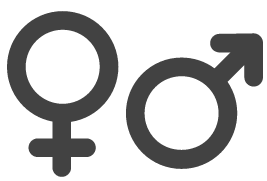
\includegraphics[width=0.3\textwidth]{pics/infographics/gender2.png}}{{\bf Male:} 529 (66\%)}}{{\bf Female} 278 (34\%)}
      }
      \hspace{0.5cm}
      \subfigure{
        \stackunder[5pt]{\stackunder[5pt]{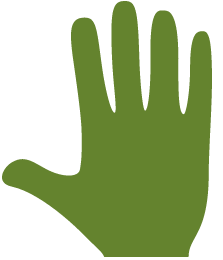
\includegraphics[width=0.20\textwidth]{pics/infographics/hand.png}}{{\bf Right:} 690 (88\%)}}{{\bf Left:} 97 (12\%)}
      } 
    \end{figure}
    
    \begin{figure}[H]
      \centering
      \captionsetup{justification=centering}
      \subfigure{
        \stackunder[5pt]{\stackunder[5pt]{
\includegraphics[width=0.27\textwidth]{pics/infographics/comp2.png}}{{\bf Experience:} 470 (59\%)}}{{\bf No experience:} 332 (41\%)}
      }
      \hspace{0.5cm}
      \subfigure{
        \stackunder[5pt]{\stackunder[5pt]{\stackunder[5pt]{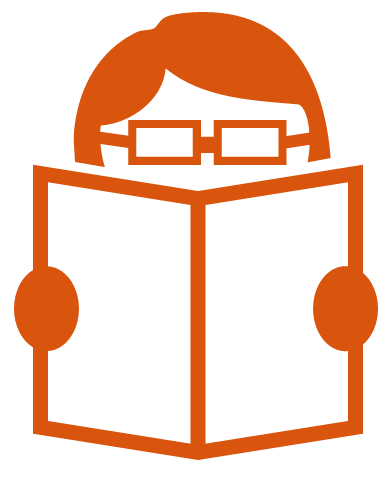
\includegraphics[width=0.20\textwidth]{pics/infographics/read.png}}{{\bf Top-to-botto:} 7 (1\%)}}{{\bf Right-to-left:} 8 (1\%)}}{{\bf Left-to-right:} 792 (98\%)}
      }
      \caption{Gender, handedness, experience with IT and security,\\ and reading/writing orientation}
      \label{fig:respondentsBasics}
    \end{figure}

    Figure \ref{fig:ageDistribution} presents a distribution of the respondents' age. The respondents are divided into 8 intervals: under 20, 20-24, 25-29, 31-34, 35-39, 40-49, over 50. The three last intervals have a lower frequency of participants, hence being grouped into smaller intervals. The distribution have a peak at the interval 20-24. Reasons for the skewed distribution can be a cause of the network that received the survey. The majority of the networks contacted were students in their twenties, hence resulting in a skewed distribution. When looking at the right-hand side of the graph, there is a lower frequency of respondents. 

    %Figure: Age distribution
    \begin{figure}[H]
      \centering
      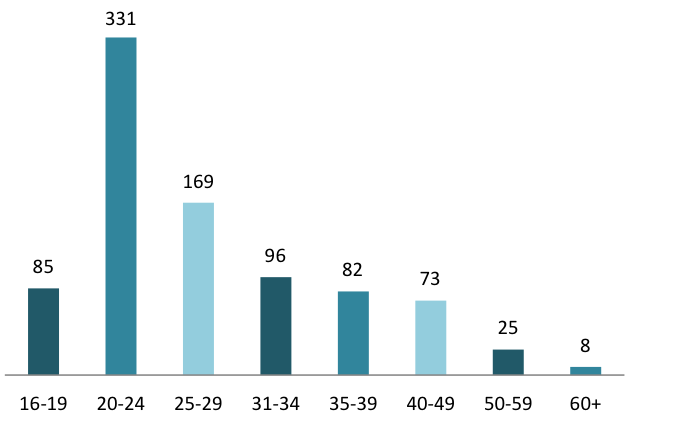
\includegraphics[scale=0.8]{pics/analysis/AgeDist.png}
      \caption{Age distribution}
      \label{fig:ageDistribution}
    \end{figure}

    Figure  \ref{fig:handsizepopulation} is the overview of the hand size of the respondents. The registered hand size is considered to be subjective and needs to be carefully used when making any conclusion. The majority of both genders classified their hand size according to their gender as a medium size. Male respondents have a higher frequency of large classifications. A more detailed quality control of the provided dataset of selected hand sizes will be carried out in Chapter \ref{sec:classificationhandsizescreensize}.

    \begin{figure}[H]
      \centering
      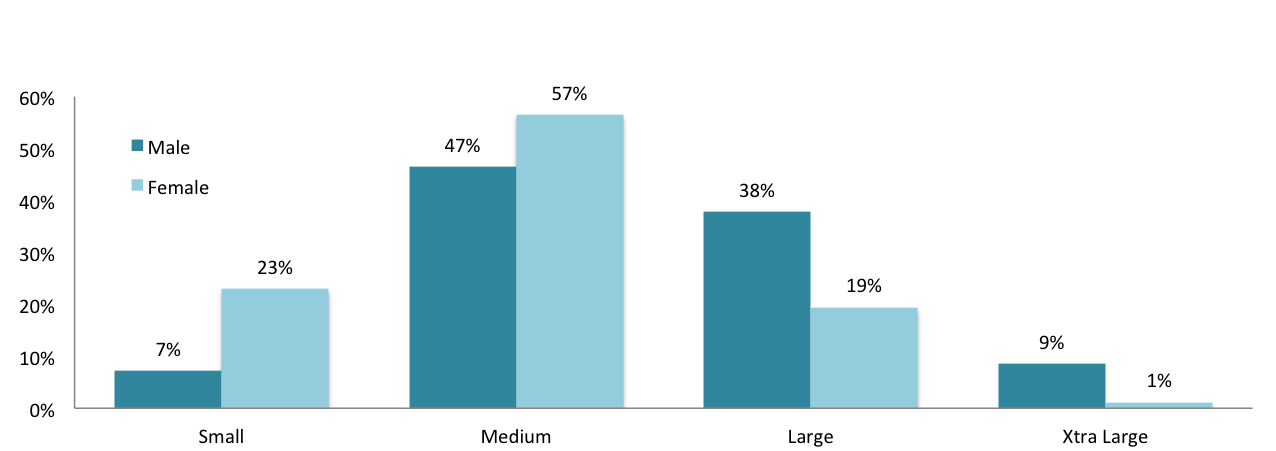
\includegraphics[width=\textwidth]{pics/infographics/mobilesize.png}
      \caption{Handsize}
      \label{fig:handsizepopulation}
    \end{figure}

    The survey asked the participants about their country of origin and the population ended up being represented by 39 countries. The majority of the countries represented in the dataset was Norway and United States of America as seen in Table \ref{tab:country}. The table summarizes all 39 countries, as well as the frequency of respondents from each of the countries. The distribution can not be used for making any conclusion of selection of graphical passwords based on the country of origin, as many of the countries represented in the population do not provide sufficient mounts of data. During the data collection it was a goal to avoid a homogeneous dataset. The majority of the participants is still from Norway, but is was important to get other countries represented as well to obtain as a more heterogeneous data set.  

   {\renewcommand{\arraystretch}{2}%

    \begin{table}[H]
      \centering
      \begin{tabular}{ l c | c }
        \hline
        \multicolumn{2}{c|}{\bf Country} & {\bf \# Respondents} \\ \hline
        \raisebox{-.4\height}{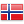
\includegraphics[scale=0.4]{pics/flags/Norway.png}} & Norway & 517 \\ \hline
        \raisebox{-.4\height}{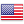
\includegraphics[scale=0.4]{pics/flags/USA.png}} & United States of America & 115 \\ \hline
        \raisebox{-.4\height}{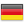
\includegraphics[scale=0.4]{pics/flags/Germany.png}} & Germany & 33 \\ \hline
        \raisebox{-.4\height}{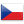
\includegraphics[scale=0.4]{pics/flags/CzechRepublic.png}} & Czech Republic & 31 \\ \hline
        \raisebox{-.4\height}{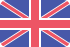
\includegraphics[scale=0.4]{pics/flags/UnitedKingdom.png}} & United Kingdom & 22 \\ \hline
        \raisebox{-.4\height}{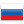
\includegraphics[scale=0.4]{pics/flags/Russia.png}} & Russia & 13 \\ \hline
        \raisebox{-.4\height}{
\includegraphics[scale=0.4]{pics/flags/Denmark.png}} & Denmark & 7 \\ \hline
        \raisebox{-.4\height}{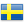
\includegraphics[scale=0.4]{pics/flags/Sweden.png}} & Sweden & 6 \\ \hline
        \raisebox{-.4\height}{
\includegraphics[scale=0.4]{pics/flags/Switzerland.png}} & Switzerland & 6 \\ \hline
        \raisebox{-.4\height}{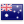
\includegraphics[scale=0.4]{pics/flags/Australia.png}} & Australia & 5 \\ \hline
        \raisebox{-.4\height}{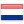
\includegraphics[scale=0.4]{pics/flags/Netherlands.png}} & Netherlands & 4 \\ \hline
        \raisebox{-.4\height}{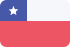
\includegraphics[scale=0.4]{pics/flags/Chile.png}} & Chile & 4 \\ \hline
        \raisebox{-.4\height}{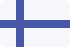
\includegraphics[scale=0.4]{pics/flags/Finland.png}} & Finland & 3 \\ \hline
        \raisebox{-.4\height}{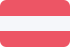
\includegraphics[scale=0.4]{pics/flags/Austria.png}} & Austria & 3 \\ \hline
        \raisebox{-.4\height}{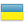
\includegraphics[scale=0.4]{pics/flags/Ukraine.png}} & Ukraine & 3 \\ \hline
        \raisebox{-.4\height}{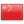
\includegraphics[scale=0.4]{pics/flags/China.png}} & China & 3 \\ \hline
        \multicolumn{2}{p{8cm}|}{Afghanistan, Mexico, North Korea, Pakistan, Vietnam, Luxembourg, Ireland, Tunisia} & 2 \\ \hline
        \multicolumn{2}{p{8cm} |}{Italy, Greece, Belgium, Indonesia, Malaysia, Bahrain, Botswana, Argentina, Singapore, japan, Canada, South Korea, Hungary, Turkey, Brazil} & 1 \\ \hline
      \end{tabular}
      \caption{Respondents country of origin}
      \label{tab:country}
    \end{table}

  {\renewcommand{\arraystretch}{1}%

  \clearpage
  \subsection{Screen Lock Habits and Mobile Device Used}
   Table \ref{tab:screenlockHabits} summarizes the respondents habits when selecting screen lock, particularly their use of screen lock mechanisms, and which screen lock they are currently using. The table also lists information about the mobile device used for answering the survey, like screen size and mobile operating system. The table provides as an overview of how the respondents manage the security on their smartphones. 

  The majority have answered the survey using a mobile running on Android or iOS that are the two most popular mobile operating systems in the market. Together, 98\% of the mobile operation system used were either Android or iOS,  constituting 58\% and 40\% of the smartphones, respectiveley.

  A total of 65\% of the participants had used the Android Pattern Lock before while 35\% of the population were not familiar with the Android Pattern Lock. The respondents not familiar with the utilization of the Android Pattern Lock will probably have their first time using the scheme in this survey.

  Looking at the screen lock habits in the population, 82\% of the participants uses screen lock on their mobile device. Among the listed screen locks in Table \ref{tab:screenlockHabits}, the majority are using either 4-digit PIN (36\%),  Android Pattern Lock (31\%) and fingerprint (18\%). The fingerprint is only available on iOS while Android Pattern Lock are not allowed on iOS. Beside the different screen locks, the mobile devices do also have different screen sizes. The stated screen size by the respondents is a subjective classification of the screen size. Further validation of the screen size and classification of correct physical size are being found in Section \ref{sec:classificationhandsizescreensize}.

    %Table: Summary of the background information
    \begin{table}[H]
      \parbox{.48\linewidth}{
        \centering
        \begin{tabular}{ l | l l }
          \hline
          \multicolumn{3}{l}{\bf Screenlock in use} \\ \hline
          Android Pattern Lock & 202 & 31\% \\
          4-digit PIN & 237 & 36\% \\
          Fingerprint & 116 & 18\% \\
          Password & 44 & 7\% \\
          slide-to-unlock & 28 & 4\% \\
          Other & 28 & 4\% \\ \hline
            
          \multicolumn{3}{l}{\bf Screensize} \\ \hline
          Small & 108 & 13.3\% \\
          Medium & 532 & 65.4\% \\ 
          Large & 173 & 21.3\% \\ \hline
        \end{tabular}
      }
      \hfill
      \parbox{.48\linewidth}{
        \centering
        \begin{tabular}{ l | l l }
          \hline
          \multicolumn{3}{l}{\bf Mobile Operating System} \\ \hline
          Android & 464 & 58.0\% \\
          iOS & 321 & 40.0\% \\
          Windows & 16 & 1.9\% \\
          Blackberry & 1 & 0.1\% \\ \hline

          \multicolumn{3}{l}{\bf Use screenlock} \\ \hline
          Yes & 655 & 82\% \\
          No & 149 & 18\% \\ \hline

          \multicolumn{3}{l}{\bf Used Android Unlock Pattern} \\ \hline
          Yes & 526 & 65\% \\ 
          No & 278 & 35\% \\ \hline
        \end{tabular}
      }
      \caption{Information about password habits and mobile device used}
      \label{tab:screenlockHabits}
    \end{table}

  \clearpage
  \subsection{The Created Patterns}\label{sec:thecreatedpatterns}
    % (\#Persons used training) & 658 

    This section is looking at the patterns created, and how the patterns were being created due to the hand and finger used. Table \ref{tab:thecreatedpatterns} summarizes the number of patterns created of the different pattern types. There is about the same abount of patterns created for all pattern types. The cause of not having the exact number of each pattern is because some of the respondents did not complete answering the entire survey as listed in Table \ref{tab:thecreatedpatterns}.

    The number of training patterns are larger than for the other pattern types because the respondents were able to create as many pattern as they liked. A total of 658, constituting 80\% of the population, created at least one pattern in training mode. The total number of patterns collected for shopping account, smartphone, banking account, and training was 3393 patterns. The distinct number of pattern created for the different types as summarized in Table \ref{tab:thecreatedpatterns}.

    On the right side of Table \ref{tab:thecreatedpatterns}, a summary are provided of how the respondents created the patterns. By observing normal interaction with a smartphone, the majority of people fall under two main categories in how to interact with a smartphone:

    \begin{enumerate}
      \item Use one hand using the thumb for interaction, whereas the hand are defined by handedness.
      \item Use the opposite hand defined by handedness and use the forefinger on the other hand for interacting with the screen.
    \end{enumerate}

    There are also people interacting with the screen using other fingers than the thumb and forefinger, hence provided an option for selecting otherwise. The majority of the respondents was either using their right hand using their thumb or using their left hand and their forefinger. Handedness may influence these numbers, hence provided more information of the pattern creation process in Section \ref{sec:subgroupHandedness} by lookig futher at handedness, hand used, and finger used. 

    \begin{table}[H]
      \centering
      \parbox{.45\linewidth}{
        \centering
        \begin{tabular}{ p{3cm} | p{1.5cm} }
          \hline
          \multicolumn{2}{l}{\bf Patterns created} \\ \hline
          Shopping & 841 \\
          Smartphone & 842 \\
          Bank & 838 \\
          Training & 872 \\ \hline
          Total & 3393 \\ \hline
        \end{tabular}
      }
      \hfill
      \parbox{.5\linewidth}{
        \centering
        \begin{tabular}{ l l | l l}
          \hline
          \multicolumn{4}{l}{\bf Hand and finger used} \\ \hline
          Left hand & Forefinger & 233 & 28.8\% \\
          Left hand & Thumb & 60 & 7.4\% \\
          Right hand & Forefinger & 72 & 8.9\% \\
          Right hand & Thumb & 398 & 49.3\% \\
          Other & & 45 & 5.6\% \\ \hline
        \end{tabular}
      }
      \caption{Information about the collected patterns}
      \label{tab:thecreatedpatterns}
    \end{table} 
